\fancyhead[LO]{{\scriptsize {\FA }我们最幸福 {\FA } 03 真正的信徒}}%奇數頁眉的左邊
\fancyhead[RO]{\thepage}
\fancyhead[LE]{\thepage}
\fancyhead[RE]{{\scriptsize {\FA }我们最幸福 {\FA } 03 真正的信徒}}%偶數頁眉的右邊
\fancyfoot[LE,RO]{}
\fancyfoot[LO,CE]{}
\fancyfoot[CO,RE]{}
\chapter*{03 {\FA } 不洁之血}
\addcontentsline{toc}{chapter}{\hspace{5mm}03 {\FA } 真正的信徒}
\begin{figure}[!htbp]
	\centering
	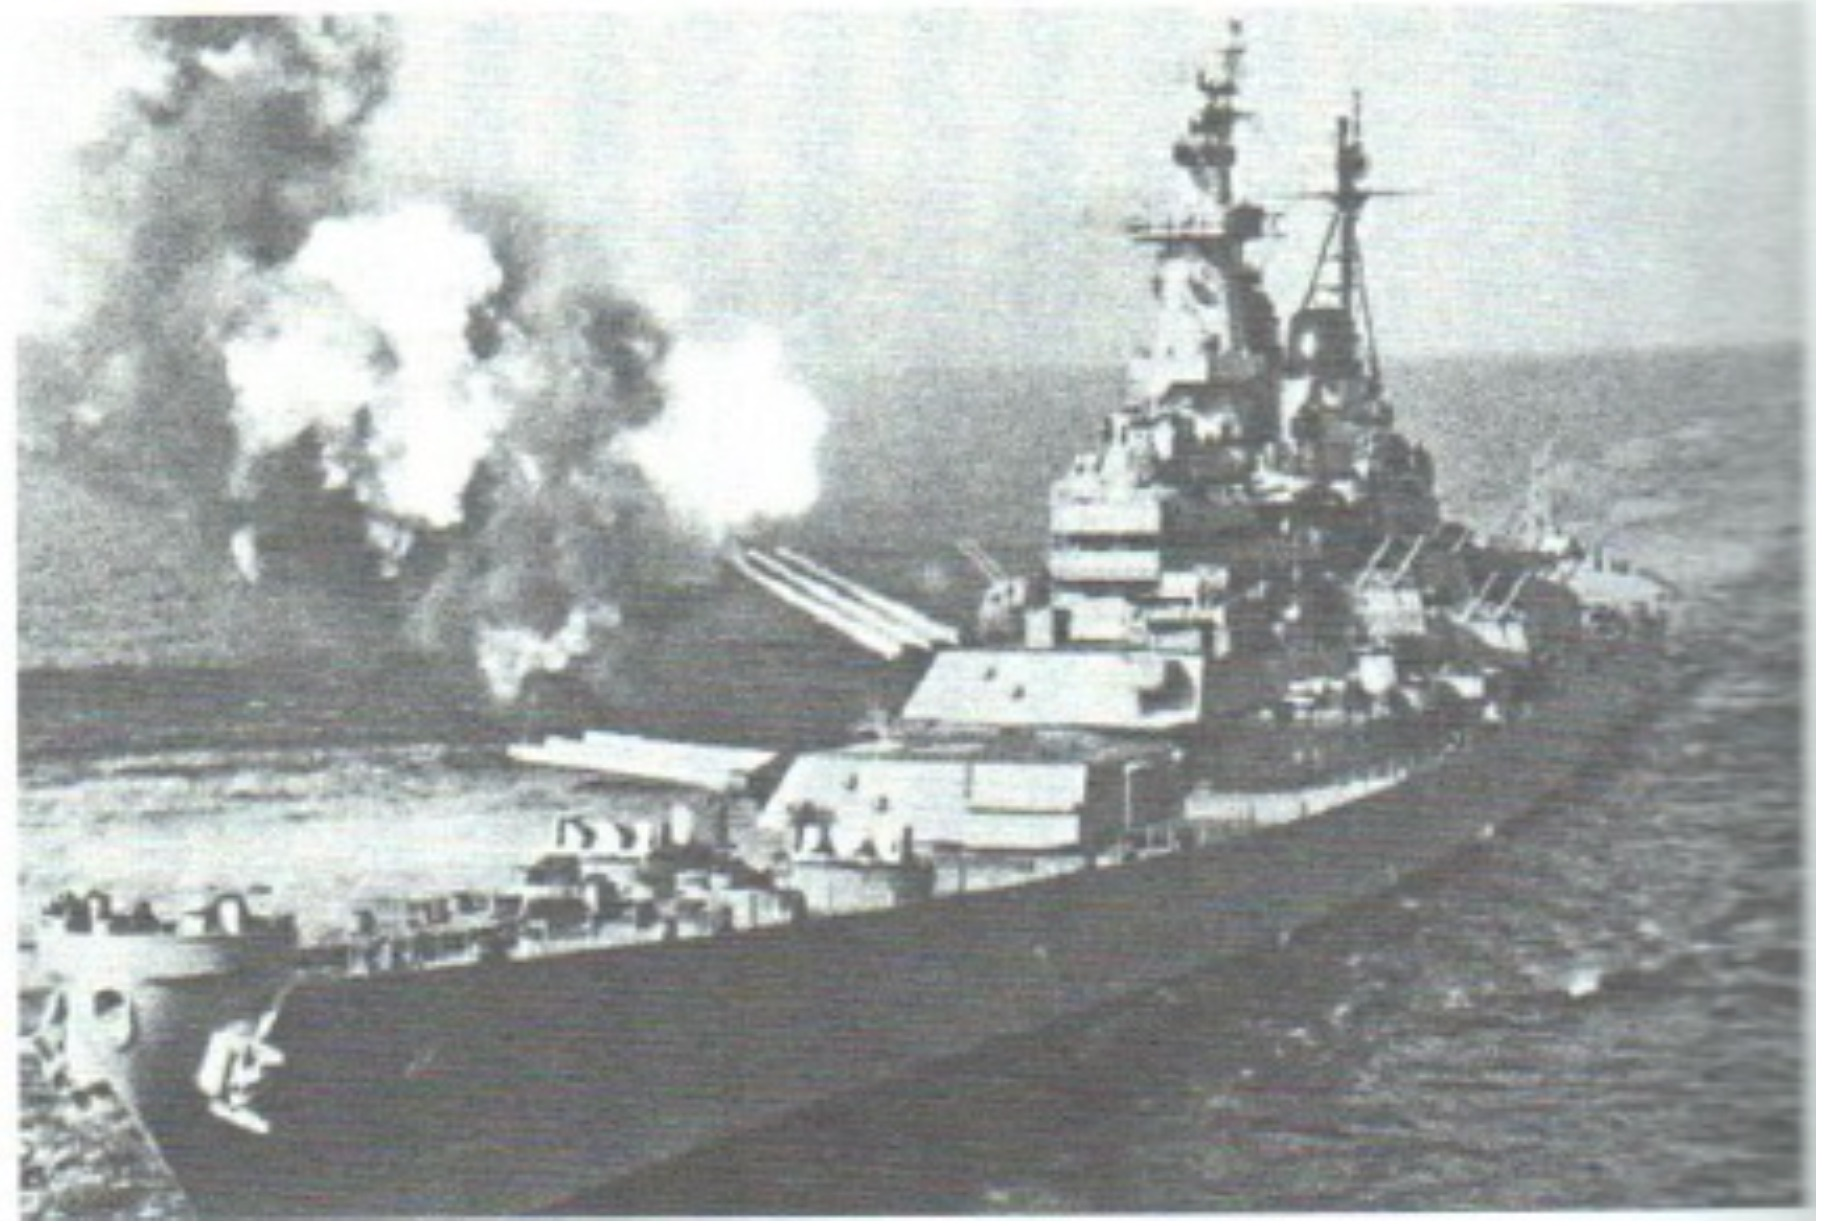
\includegraphics[width=6cm]{./Chapters/Images/03.jpg}
	\caption*{1950年10月美国密苏里战列舰炮轰清津}
\end{figure}

清津这个城市有着不太好的名声,自然条件十分恶劣,即使按照北朝鲜的标准,也没什么人愿意选择居住在这座城市。这个城市的50万居民就见缝插针的挤在山脊与蜿蜒的东海海岸线之间那一片狭长的地带。沿着海岸线,礁石密布,景色非常美丽,波光粼粼之下,是一片幽深刺骨的海水,然而,这也意味着如果没有坚固的渔船,打渔将变得非常危险。山间终日的狂风使得地里长不出什么庄稼,冬天气温也会降至4度以下。只有沿着海岸,地势低洼的地方可以种植水稻,大米不仅仅是朝鲜人的主食,还是朝鲜文化的精髓,一切都围绕大米展开。历史上,朝鲜人衡量成功的标准之一就是你离权利中心的距离,这也是亚洲的一个悠久传统,人们都想远离穷乡僻壤的乡下,来到皇城根儿的脚下。清津几乎位于朝鲜版图之外,是朝鲜最北的一个城市,以至于从清津到俄罗斯远东城市海参崴比去平壤近多了。时至今日,清津至平壤之间直线距离仅仅400公里,汽车却要在砂石路面的山路上,蜿蜒盘旋上3天3夜。\\

在朝鲜李朝时期,首都甚至更远,位于大致相当于现在首尔的位置,那些惹恼国王的大臣们都被发配到清津──这个王国的化外之地。因而,这个地方的人,往往都有着天生的桀骜不驯。到现在,出生于咸镜北道的朝鲜人,被认为是朝鲜人当中,最能吃苦耐劳,也最坚强不屈的。\\

咸镜北道,是位于朝鲜最北部的省份,一直向北延伸至图们江──朝鲜同中国及俄罗斯的界河,直到20世纪,其人口稀少,经济上也无足轻重。再早几个世纪,可能那里老虎的数量都比人多,在很多朝鲜的传说故事里面,经常出现的老虎至今仍然吓唬着孩子们。今天,老虎早以销声匿迹了。随着日本人在朝鲜王宫上插上了日本国旗,这里一切都改变了。咸镜北道位于日本人通往满洲的必经之地,而占领满洲是日本人发动全面战争的先决条件。不仅如此,日本人还对位于茂山一带几乎未开采的煤矿、铁矿垂涎已久,他们需要将这些战利品从半岛运回日本。清津(Chongjin)\footnote{这个名字来源于中文,意思是清澈的渡口。}这个小渔村,也就发展成为一个港口,每年货物吞吐量达300万吨。在1910年至1945年日剧时期,日本人在清津建了大型钢厂,在更南的地方,他们发展了罗南,一个有着横平竖直的街道,规划的非常整齐的现代化城市。曾参与侵略中国华东地区的日本帝国陆军第19师团将司令部设在这里。沿海岸线再往南,日本几乎从无到有,建立起了咸兴市,这里集中了很多大型化工厂,生产着从火药到化肥等各种产品。\\

50年代,共产党上台之后,他们重建了在战争期间屡遭轰炸的工厂,并冠以自己的名字。清津的日本钢铁变成了金策钢铁,成为北朝鲜规模最大的工厂。该工厂也被金日成亲自点名,作为北朝鲜工业实力的代表,成为在他领导下经济所取得的光辉成就的示范。今天,清津市的居民对于这个城市的历史知之甚少──事实上,这个城市看上去根本没有过去──北朝鲜政权对日本人在这些城市发展中所做的贡献是不会有任何的正面评价的。到了朝鲜民主主义人民共和国时期,由于名声和人口都有所提升,使得清津于70年代成为朝鲜第二大城市,人口几近90万\footnote{近期,清津人口相信有所下降,估计在50万左右,成为排在咸兴之后,北朝鲜第三大城市。}。\\

清津,有时也称之为“钢铁之城”,籍着所拥有的钢铁工业,成为越来越重要的经济和战略重镇。那里的工厂出产手表、电视、人造纤维、医药、机械工具、拖拉机、农具、钢铁板材及军需品。渔业捕获的海蟹、鱿鱼以及其它海产品都用于出口。港口也被用于造船。沿着海岸线,从上到下,原来日本人的军事设施都被北朝鲜人接管,建成瞄准日本的导弹基地。不变的是,清津周围的农村继续成为敌对阶层和动摇阶层的流放地,像美兰的父亲,就被安置在一个矿业小镇。然而,这个城市又是如此重要,绝不能落入不可靠的人手里。这个政权需要来自核心阶层,忠诚的党干部执掌这个城市,确保清津时刻同党保持一致。因而,清津有着一个掌权的精英阶层。他们都住的很近,然而不是紧紧的挨着,中间还加扎着些被踢出这个精英阶层的失势者。处于北朝鲜社会阶层两个极端的人,在同一个地方交织在一起,就其本身就赋予清津一种特有的活力。\\

宋熙锡是一个不折不扣的共产主义信仰者。作为一个工人,也是四个孩子的妈妈,她是北朝鲜的模范市民。她可以滔滔不绝的复述着金日成的语录,对其内容她也是深信不疑。她是个非常循规蹈矩的人。宋女士\footnote{她是这么称呼自己,北朝鲜的妇女婚后并不改随夫姓。}对这个政权是如此的爱戴,以至于她看上去像是宣传影片里的英雄式的女主角。在年轻的时候,她也确实有点像,然而在那个时候,谁又不是这样的呢?她天生就长了一张金正日式电影的脸:她面相饱满,让人看不出营养不良;微翘的嘴角,使人读不出内心忧郁。小小的鼻头光亮亮的,加上诚挚的目光,使得她看上去真诚热情──事实上她也确实是。\\

就一切事实而言,很明显这个体系辜负了她,但是她仍然保持信念,毫不动摇。“我只为金日成将军和祖国而活着,别无他念”,我们第一次见面是,她是这样告诉我的。\\

宋女士出生于二战的最后一天,1945年8月15日。她在清津市火车站附近长大,当时她父亲是位铁路工人。朝鲜战争爆发后,铁路成了美国主导的联合国军重点的打击对象,以掐断共产党军队沿着海岸的补给线和交通线。美国海军战列舰密苏里号及其它战舰云集日本海海域,炮轰清津及其它海滨城市。不时在头顶盘旋的美国军机,吓坏了孩子。有时候他们飞的如此之低,以至于宋女士可以清楚的看到飞行员。白天的时候,宋女士的母亲为了孩子们的安全,拉着六个孩子躲进山里。夜晚的时候,他们就会回来,睡在邻居们在房子外面挖的避难处。这时候,宋女士总是在薄毯之下,瑟瑟发抖,紧紧的挨着母亲和其它兄弟姐妹。一天,宋女士的母亲丢下孩子,去打探她父亲的情况。因为就在前一天晚上,清津遭到猛烈空袭,一个生产铁路部件的工厂遭到摧毁。她回来的时候泪流满面,长跪着以头呛地,哭道:“孩子他爸被炸死了。”此时孩子们围着母亲哭成一团。\\

父亲的死使宋女士成为根红苗正的“祖国解放战争烈士”子女。家里得到政府颁发的证书。父亲的死也在她心里烙下深深的反美主义情绪,同时这也是这个国家意识形态的主旋律。在人生中易受影响的那几年经历着战争的混沌后,现在她准备接受在劳动党安排下,有条不紊的生活。并且,她家里也非常穷,理所应当有资格成为金日成声称所代表的受压迫的下层劳动人民中的一员。有着如此纯正共产主义信仰的女孩,当然只有选择门当户对的,婚姻才能称得上完美。她的未婚夫,长博也是劳动党党员,她也从未想过同一个不是党员的人结婚。长博的父亲作为一个情报特工,在战争中表现突出;他的弟弟当时也已供职于北朝鲜公安部。长博毕业于金日成大学,是个记者,这可是在北朝鲜倍受尊敬的职业,因为记者可是这个政权的喉舌。“那些按照党的意志写报导的记者都是英雄。”金正日就曾这样说过。\\

长博身材魁梧,在他那一代北朝鲜人里面属于异常高大的。宋女士只有150公分高,依偎在长博的身边,长博的搂着她,显得她是那么的小鸟依人。多么完美的一对啊!这对政治上正确的俊男靓女是很容易获得居住在平壤的资格的。因为平壤是北朝鲜唯一的经常有外国人造访的城市,因而这个政权也尽其所能,保证平壤的居民能以他们良好的外表及精神面貌给访问者留以深刻印象。然而,上级决定这对夫妇需要回到清津,以巩固那里的精英阶层,因此他们定居于清津,住在有一定特权的,最好的小区里。\\

在北朝鲜,一切都是平均主义,住房也是按照背景、成分等级来分配。在清津,没什么人要住在南边的住宅区,那里靠近煤矿和高岭土矿。房子也都是些刷着白灰低矮的口琴屋。北边的情况就好多了。一条大道穿过罗南,建筑也比南边高多了,有些住宅楼高达18层,在当时建造的时候,算是很现代化的了。建造者们甚至给这些建筑留下了安装电梯所需要的主轴,虽然他们从来没有考虑会由他们自己来安装电梯。很多战后公寓楼建筑设计的思想都来自于东德,并根据朝鲜文化做了相应的修改。楼层之间增加了额外的夹层,以容纳朝鲜的一种地暖系统。每一个房间都安装有扬声器,用于播放小区通知。\\

清津远离着现代化的平壤,但是这个城市也有自己的特权阶层。作为咸镜北道的省会,清津有着一个很大的省委省政府办公区。以这个办公区为中心的城区规划的十分整齐,附近区域设有一个大学、一个冶金学院、一个矿业学院、一个农学院、一个艺术学校、一个外国语学院、一个医学院、三个师范学院、十几个剧院,还有一个革命历史博物馆。东边港口对面是专门接待外宾的天马山宾馆,宾馆旁边是俄罗斯领事馆。城市的街道广场都被设计成夸张的巨大,气势非常恢宏,属于那种莫斯科或其它共产主义城市流行的风格,处处体现着这个政权掌握着的,那种凌驾于个人的无上权力。\\

贯穿整个城市的第一大道,可以轻而易举的容下6车道,不过前提是清津要有这么多车辆。路两侧,每隔一定的距离就有着像卫兵一样竖立着的行道树,主要是松树和洋槐,树干下半部都涂成白色。关于为什么要涂成白色有很多说法,一般认为是为了防虫蛀、保温,还有人说是给树做标记,即为政府资产,不得私自砍伐以作柴火。路沿石也被涂成白色。树木之间点缀着无处不在的写着革命口号的红色标语牌。标语牌后面,是高高的路灯,然而现在却鲜有点亮之时。沿着车道设有同香榭丽舍大街一样宽阔的人行道,虽然有这么好的林荫大道,但是因为路上没什么车,多数行人还是直接走在车道上。路上没有交通信号灯,只有穿着制服的警察,像跳着机器人舞一样,挥舞着胳膊指挥寥寥无几的交通。大路在咸镜北道大剧院前就到了头,这是个宏大的建筑,顶上有一副高达3.6米的金日成画像。剧院后面,这个城市突然来到了尽头,Naka山由此一直向着东北方向蜿蜒。如今,山坡上星星点点的到处是坟墓,树都被当成柴火大多被砍光了,然而这里仍然景色宜人,不失为一个休闲的好去处。事实上,就清津的主城区而言,即使今天看来,也能给访客留下良好印象。然而所有的这一切,都只可以远观,如果细察,你就会发现,建筑物上大块混凝土剥落,街灯七倒八歪的斜着,有轨电车上满是是坑坑洼洼,但是对于数量有限的那些访客而言,对这个城市也就是一闪而过,所有的这一切都很轻易的被忽略掉。\\

宋女士的新家位于一幢8层楼房的第二层,没有电梯。当宋女士第一眼看到房子的时候,她惊奇的发现,房间里有室内管道系统──像她这样的普通人在60年代是从没见过如此先进的设备。房间的取暖通过加热地板实现,一如朝鲜传统住宅,不同的是热源来自热电厂通过管道系统送来的热水。小夫妻当时没有什么家具,但是他们却有两个房间,一间他们自己住,另外一间给数量不断增加的孩子们住。他们的第一个女儿──玉熙出生于1966年,2年后又生了个女儿,之后还是个女儿。北朝鲜当时医疗水平有较大发展,大多数城市的妇女都是在医院生孩子,但是宋女士外表看上去是除此柔弱,然而内心却是坚强无比。她所有的孩子都是自己在家生的,甚至连接生婆都不要。有一个孩子还是在路边生的,当时她挎着一篮子洗好的衣服走在回家的路上。当她生第一个孩子的时候,她婆婆给她炖了海带汤,一种朝鲜人专门为产妇补铁的偏方。第二次,婆婆只是把海带扔给她,让她自己煮。再生了三个姑娘之后,她婆婆再也不理她了。\\

“你注定就生不出个带把的。”她临走的时候只丢下这句话。\\

宋女士并不气馁,第四个孩子出生的那天下午,她当时独自一人在家。那天,她因为肚子疼就早点回了家,在家里她也闲不住,就开始擦地板。这个时候,肚子一阵剧痛,她意识的可能要生了,马上冲进了厕所。一个男孩,谢天谢地,终于是个男孩。宋女士在家里人面前又挺直了腰杆。这次她婆婆亲自下厨给她炖了海带汤。\\

长博当时正在外地出差,第二天才得到消息。他立刻搭第一班火车往家里赶,半路上停下来买了一辆儿童自行车──送给尚未谋面的儿子的礼物。\\

除了照顾4个孩子和操持家务,宋女士还要完成自己的全职工作,作为在位于浦项(Pohang)的朝鲜制衣厂附属日间看护中心的财务人员,她一周需要工作6天。在北朝鲜,女人们是维持工厂运作的主力军──因为男人总是不够──大约20\%的适龄男性在军队服役,按人均来看,是世界上军人比例最高的国家。为了照看孩子,宋女士工作时,通常背上背着一个,手上还要牵着一两个。她的孩子也基本上都是在日间看护中心长大的。按照规定,工时为8小时工作制,期间有一个午餐时间,和一个班间休息时间。下班之后,她还要去工厂的礼堂参加几个小时的政治学习。某一天的主题可能是关于如何同美帝国主义作斗争,而另一天可能是金日成的在二战期间反抗日本的丰功伟绩(或真实,或夸大其词)。不仅如此,她还要就劳动党最新声明,以及《咸镜日报》的社论完成自己的思想汇报。这样,当回到家的时候,几乎就是晚上10:30了。然后还要做家务,煮饭。第二天,天不亮就要起床,赶在全家人7点钟离开家之前,准备好所有人一天的饭菜。因此,宋女士很少有能睡5个小时以上的时候。某些天,要比平时还要紧张。在周三的早上,她要比平时更早到单位,参加的社会主义妇女联合会的周会。周5的晚上,则是自我批评的时间。这时候,单位的同事就轮流站在大家面前进行自我批评,坦白自己的工作失误。这个是共产主义版本的忏悔。宋女士这个时候一般都饱含真情的责备自己工作的还不够努力。\\

宋女士对自己的话是心口一致的。多年的睡眠不足,多年的自我批评──这些与洗脑或审讯如出一辙的手法,使得宋女士连反抗的念头都未曾冒过。她已经被塑造成按照金日成所设想的人类改造的楷模。金日成的目标不仅只是建立一个新国家;他还想打造一个全新的人民,重塑人性。以此为目的,他创造了自己的哲学体系,主体思想,一般也解释为“自力更生。”主体思想,汲取了马克思列宁主义关于地主与农民,富人与穷人之间所存在的阶级斗争的思想。它也相类似的宣称,是人而不是神主宰着自己的命运。然而,金日成又剔除了一般意义的共产主义所倡导的消除国家以达到大一统的国际主义观点。金日成是个极端的朝鲜民族主义者。他不断向人们灌输着,北朝鲜人民作为一个几乎是被精心挑选出来的民族,从今以后不再需要仰中国、日本或俄罗斯等强邻之鼻息。而南韩毫无尊严,简直就是美国人的走狗。“简而言之,建立主体思想,依靠自身的力量成为开展革命与国家重建的主人,向世人展现以自力更生的革命精神。”金日成在其众多的文章中的一篇中是这样解释的。这种说法对于一个几个世纪以来,尊严被邻国反复践踏,而内心又十分高傲的民族来说,无疑是极具诱惑力的。\\

一旦掌权,金日成完善了在抗日游击战争过程中形成的思想,并将其发展成为一种社会控制手段。他指示北朝鲜人,个人的力量是有限的,然而将个人融入集体,那么所展现的力量是无穷的。然而,集体也不能不容分辨的按照人们的意志行事,即使这是经过某种民主过程而确定下来的。人们应该毋庸置疑的听从一个绝对的最高领袖的指导。这个领袖毫无疑问就是金日成自己。\\

然而,这还不够。金日成还想被爱戴着。在鲜艳的宣传画中,他被一群面色红润的孩子簇拥着,孩子的目光里充满着敬意,好似他们洁白的牙齿,开怀的大笑全部都是拜他所赐。玩具,自行车占据这画面的背景──金日成不想做约瑟夫斯大林;他要做圣诞老人。他那张带着酒窝的脸也使他看起来比其它的独裁者更和蔼可亲。他被北朝鲜人尊称为父亲,而在儒家文化里,父亲意味着威严和慈爱。他希望人们视他为挚爱血亲,自家人。这种儒家共产主义很类似与日本军国主义的观点,认为天皇即为万物之源的太阳,这同卡尔马克思的初衷可谓大相径庭。\\

在有的方面,所有的独裁政权都是一样的。从斯大林的苏联,到毛的中国,从齐奥塞斯库的罗马尼亚到萨达姆侯赛因的伊拉克,所有的这些政权都有着同样的嗜好:独裁者的雕像俯视着几乎每一个广场,他们的画像挂在每一间办公室,甚至腕表的表盘上都是他们的脸。但是金日成却把个人崇拜推向一个前所未有的极致。在20世纪独夫的群丑图中,他驾驭信仰的能力,也使他区别于其它独裁者。金日成了解信仰的能力。共产党时代之前,他叔叔是平壤一个基督教牧师,而当时平壤的基督教小区也颇具规模,以至于曾被成为“东方的耶路撒冷。”甫一上台,金日成就关闭教堂,查禁圣经,信众也被发配苦寒之地,然而对基督教传教所用的图像膜拜,宣讲布道的方式,却被他盗取,将这套手法用于对自己的自吹自擂上面。\\

广播里,播音员以一种几近宗教崇拜的方式连篇累牍的报导着金氏父子,其密集程度简直令人窒息。报纸上也不厌其烦的报导些超自然现象的故事。当抓住倾覆的船沿,在水里挣扎的水手唱起金日成的赞歌时,怒海奇迹般的平静下来。当金正日来到位于朝韩边界的非军事区时,一团神秘的浓雾骤然升起,保护着他免遭敌人的冷枪袭击。他使铁树开花,冰雪融化。如果金日成是上帝,那么金正日就是上帝之子。一如耶和华的诞生,据称,金正日诞生之时,繁星闪耀,天空出现七彩虹霓,一只神雀从天而降,口中唱着“征服世界的将军啊。”\\

北朝鲜政府的这一套实在称不上高明。我们嘲笑那些拙劣的宣传手法,嘲笑他们的愚昧。然而,如果考虑到他们从摇篮就开始被灌输着这些教化,一天14个小时的工作,重复50年,每一首歌曲、电影、报导、标语牌都在歌颂着金日成,外界关于神一样的金日成的任何质疑都被严格的屏蔽着,在这样的环境下,谁又能保证他们能抵御这些呢?\\

1972年,金日成60大寿,在朝鲜文化中,60是人生中一个重大的时刻,劳动党开始分发金日成像章。不久之后,全民都被要求将这种像章佩戴与左胸,略高于心脏的位置。在宋女士家中,其它人也都一样,在一面空着的墙上悬挂装裱精美的金日成画像。悬挂着画像的那面墙不允许再放置其它的东西,即使是亲人的照片也不允许。金日成就是你唯一家人,至少在80年代只这样的,之后在金正日当上劳动党总书记之后,他的画像也被挂在了他父亲的旁边。再后来,挂上了第三个画像──父与子的合影。北朝鲜的报纸也开始报导这“闪着人性光辉的故事”,那些英雄的人们,为了保全这些画像免于火灾或者洪水的吞噬,而献出生命。这些画像都是由劳动党免费发放,且随画像包装盒里附带一块白布。按照规定,这块白布只能用于清洁画像。这在雨季显得尤为重要,以为在雨季的时候,会有霉菌从画像镜框的边角开始滋生。而且,来自公共标准监察部的检查人员也会一个月一次定期的来检查画像的清洁情况。\\

宋女士不需要为应付监督而清洁画像。即使在分秒必争的早上,卷起被褥,准备早饭,催促孩子们出门,她仍然不忘将画像快速的擦拭一边。有些妇女不喜欢佩戴像章,因为那样会在衣服上戳出一个洞,而且有时候还会留下锈迹,但是宋女士从不忘记佩戴。只有一次,她因为换好衣服匆忙出门而忘记了,在路上,背一个带着红袖标的,属于社会秩序维持队的一个十几岁的孩子拦住。这是共青团所设立的专门检查人们佩戴像章情况的检查岗。第一次违反,通常要被强制参加政治思想学习,并且在个人档案里留下不良记录,但是,宋女士非常诚惶诚恐的意识到自己的疏忽,以至于那个孩子只是给了个口头警告就让她离开了。\\

宋女士的生活完全按照她在工厂的晚间政治学习中所学到的领袖的教导来展开。甚至在她日常的对话都会出现领袖的语录。“忠诚和孝道是革命者的最高境界”是她在教训那些顽皮的孩子时最常用引用的句子。同其它北朝鲜的孩子一样,宋女士的孩子并不过他们自己的生日,然而却庆祝领袖们的生日,金日成是4月15号,金正日的在2月16号。这两个日子也是国家法定假日,也是他们家唯一能分到肉的日子。后来,在能源短缺的日子里,也是唯一有电的日子。在每个生日之前的几天,劳动党给每个孩子分发大约1公斤的糖果。对孩子们来说,这份礼物太有诱惑力了,有各种饼干,果冻,巧克力,和口香糖。这些东西没到日子之前是不能吃的,但是有些妈妈不管那么多,宋女士却不会这么做,她总是严格按章行事。当时候到了,孩子们都排列在领袖画像前,集体的向画像鞠躬,以表达他们对领袖的感激之情。\\

“感谢您,亲爱的父亲金日成。”当孩子们说这些的时候,他们的妈妈颔首微笑着。\\

多年以后,当宋女士回首这些日子时,仍然沉浸在幸福之中。她认为她还是幸运的。长博也证明是个好丈夫,他从不沾花惹草,也从来不打宋女士和孩子,就是高兴的时候爱喝两口,也总爱就着自己越来越大的肚子开玩笑。他们曾经是这样一个充满爱的幸福家庭。宋女士爱着她的三个女儿,爱她的儿子、爱她的丈夫甚至那时,她还爱她的婆婆。当然她也热爱着金日成。\\

宋女士对那些年里仅有的一些欢乐时光,始终念念不忘。周日的时候,非常难得当她和长博都不加班,孩子们也都不去学校,全家人凑在在一起。这么多年来,也就只有两次,于是全家人就一起来到离家仅仅几公里的海边。虽然没人会游泳,他们只是在沙滩上走走,挖着沙子里藏着的蚌壳,然后带回家蒸蒸就是一顿晚餐。还有一次,儿子11岁的时候,她带他去清津动物园。这个动物园,她在小时候学校组织的郊游时去过一次。她记得那时候,动物园里有老虎,大象,狗熊,还有狼。但是后来那次,动物园只剩下了几只鸟。从那以后,她就再也没有去动物园了。\\

当孩子们越来越大的时候,各种麻烦也开始接踵而至。四个孩子中,最难管教的就是大女儿,玉熙。玉熙和宋女士简直就是一个模子里刻出来的──个子不大、丰满、长得也很漂亮。虽然有着同样可爱的嘴唇,玉熙的却总是生气的撅着。她的个性乖张鲜明。和妈妈的宽容完全不同,她脾气火爆,总是那么咄咄逼人。由于妈妈需要早出晚归的在外工作,作为大女儿,她要承担很多家务,而这也让她颇有微辞。玉熙不像她妈妈那样能吃苦耐劳。她无法容忍哪些让生活变得如此折磨人的蠢事。她的叛逆并不是因为她很懒,她只是不喜欢做毫无意义的事情。\\

她讨厌“义务劳动”,那是所有北朝鲜的青少年被要求履行的爱国义务。从12岁开始,孩子们就被动员起来,成队的送到乡下,参加水稻的种植,插秧,除草。她害怕春天,每到那个时候,她就要抬着一筐筐的土,或者去喷洒那些刺眼的农药。列队行进的时候,其它孩子都兴高采烈的唱着“让我们保卫社会主义”的时候,她只是怒视着前方一言不发。\\

最让玉熙忍受不了的是要从公寓的厕所里收集“粪”。长期以来,北朝鲜一直缺乏化肥,而且也没什么家畜,因此需要收集人的粪便作为肥料。每家每户都要收集一桶,每星期一次,交到10公里之外的仓库。交完便可得到一张便条,以证明完成本周的份额,凭着这个便条,才能领到下一次的粮食配给。这个臭气熏天的苦差,通常都是由家里的老大承担,于是玉熙开始盘算着找个捷径。实际上要打歪主意也很容易。存放一桶桶粪便的仓库没人看管\footnote{毕竟谁又会去偷一桶屎回家呢?},玉熙悄悄溜进仓库,提了一桶,就当她自己的交上去,然后拿到了便条。\\

回家之后,玉熙沾沾自喜的夸耀着自己的小聪明。宋女士却被女儿的诡计彻底激怒了。一直以来,她都知道这个大女儿是四个孩子中最聪明的──她3岁就开始识字,能在亲戚面前大段的背诵金日成著作。然而这件事,证实了妈妈最担心的事情,玉熙是个缺乏集体主义精神的个人主义者。她又如何在这个追求步调一致的社会里生存啊?\\

玉熙高中毕业后,宋女士的丈夫动用自己的关系为她在一个建筑公司宣传部谋得一份差事。玉熙的工作就是写些通讯,报导超额完成任务的工人,报导公司在筑路工程中所取得的巨大进展等等诸如此类的内容。公司有个宣传车,那是一台破破烂烂的军用面包车,车两边刷着标语“让我们以主体思想规范全社会”宣传车巡回于建筑工地上,此时,玉熙在麦克风前朗读这她的通讯文章,然后声音由车上附带的扬声器广播出去。这是份轻松有趣的工作,不需要肩挑背扛,而且像其它的宣传部门的工作一样,是人们羡慕的工作。\\

为了玉熙将来生活美满,宋女士和丈夫开始为玉熙物色一个合适的丈夫。宋女士希望找一个和她自己丈夫类似的人选,于是她让长博在周围找个年轻版的自己。有一次长博出差,乘火车去茂山,和他同坐的是一个可爱的年轻人。郑永洙,来自罗津的一个良好的家庭,罗津是清津之北的一个小城。他是朝鲜人民军的文职人员,在军乐队里是个小号手。在北朝鲜,在军队有点职位和影响力的人肯定都能加入劳动党。长博想这个年轻人看上去前途光明,因此邀请他到家坐坐。\\

玉熙和永洙于1988年结婚,婚礼是典型的北朝鲜式的──在金日成雕像前举行,如西方的牧师一样,按这种方式金日成缺席主持了北朝鲜所有的婚礼。他们穿上最好的衣服──玉熙穿着米黄色的夹克和黑裤子,永洙是一套黑西装──肩并肩拘谨的站在高耸的铜像前拍了结婚照。他们在铜像面前献了花,籍此希望他们的结合能受到伟大领袖的祝福。之后,他们回到家里,享受宋女士准备好的饕餮大餐。按传统,婚宴是要吃两次──新娘家一次,新郎家一次,某种意义上也是两家显摆的一个比拼。结婚的花费是不菲的,因为要宴请邻居,同事,除此之外,娘家还要准备衣橱,及满橱的被子,全套厨具,大衣镜,及化妆台,如果家境殷实的话,嫁妆还可能包括缝纫机或者家电。宋女士有点自信心不足。她知道她的亲家──永洙的家境更好,因此她也倾尽所有,以期给亲家留下一个好的印象。她准备了满桌子的好菜──朝鲜打糕、鳕鱼、清蒸八爪鱼、油炸豆腐、毛蟹、还有三种做法不同的墨鱼干。这顿大餐可是家里有史以来最为奢侈的一顿了,也是这次婚礼最值得称道的地方了。\\

然而,婚后才发现永洙喜贪杯中之物,尤好浓酒,一种自酿的廉价米酒。几杯下肚之后,他那讨喜的音乐家的优雅就荡然无存,恶劣的嘴脸立然显现。最初让玉熙着迷的,那侃侃而谈的英俊面容在瞬间就变得恐怖可憎。这对新人婚后,搬进了位于火车站附近的新居,但是玉熙却隔三差五的跑回娘家。每次回来,不是黑着眼圈,就是豁着嘴唇。结婚后大概半年的时候,永洙应为与同事打架,被军乐团开除。他被安置在茂山一个铁矿里工作。现在,他加入劳动党的希望破灭了。在北朝鲜,如果想加入劳动党,那你就要在20多岁的时候申请,再由单位的党委书记进行考核。入不了党,永洙的前途也就堪称黯淡。而且偏偏此时,玉熙又怀孕了,孕期强烈的妊娠反应让她不得不放弃工作。她的处境比以往更糟糕了。\\

没多久,宋女士的儿子也开始让人头疼起来。与玉熙不同,他从小就是一个规规矩矩的孩子。南玉自小就是个结实的孩子,这点和他爸爸很像,长大后,他有着一身强健的肌肉,身高也有175厘米。虽然块头高大,但是他说话声音却很小,也几乎从不与人吵架。无论是父母还是姐姐们吩咐什么,他总是言听计从,毫无怨言。关于他,玉熙曾这样感叹到,真是龙生九子啊,同一个爹妈生出来的怎么就那么不一样呢?“他要是不吭声,你都不知道他在哪儿。”南玉成绩一般,但是颇有运动天赋。他最快乐的事情是自己独自玩耍,不厌其烦的一次次将球踢向公寓楼的侧墙。在11岁那年,一个体育教练给他测了前臂和腿的长度之后就把他带进了清津市体校。这是共产党政权就竞技体育选材的一套做法──通常是由国家而不是家庭决定这些孩子是不是要放弃正常学业而进入国家队进行专业体育训练。南玉也不负众望,14岁的时候就被调入平壤,接受拳击训练。\\

随后的7年里,南玉一年只能回来两次,每次两周。宋女士一年到头也见不到他几次。原本他就不像姐姐们,喜欢在妈妈怀里撒娇,现在就更是形同陌路。然而,宋女士却听见一些风言风语,外面都传开了,南玉在清津有个女友,一个大他足足5岁的女人。当他从平壤回来的时候,经常会住在那个女人的家里。这在当时简直就是个双重丑闻,一是按朝鲜传统,男人不愿同比自己大的女人交往,二则是朝鲜社会不能容忍婚前性行为。南玉因此会被体校开除的,或被逐出共青团。作为家里的独子,找个好姑娘,结婚生子,延续家族是他责无旁贷的重任。就此,宋女士和丈夫曾就此事经质问过他,但是得到的响应只是死一般的沉默。从那以后,南玉同家里就更加疏远了,有时候,即使有假期,他也不愿意回家看看。\\

随后,长博也惹上麻烦,差点吃官司。有一天晚上,他和宋女士在家同一些上门的邻居一道看电视。宋女士和她丈夫是整栋楼里少数家里有电视的人家。在1989年,电视相当于一般人3个月的工资,大概合175美元,而且没有单位的特别许可,你有钱也买不到。电视也被政府以金日成的名义奖励给那些在工作中做出杰出贡献的人。长博家里的电视是因为长博父亲在朝鲜战争期间对南韩出色的情报工作而获得的。电视是日本日立公司生产的,但是注册了一个朝鲜的商标,松树牌。电视和收音机在北朝鲜在出售前都做了设置,以确保只能收到官方的频道。尽管如此,有些电视节目还是很有意思的。除了例行公事的金日成讲话,在平时的晚上,有时候会播放体育节目、音乐会、电视剧,还有那些金正日的电影制片厂拍摄的电影。在周末的晚上,会播放特别节目,有时可能是俄罗斯的电影。宋女士和丈夫都因家里的电视而引以为豪。通常,他们都会开着门,这样邻居们可以来串门,一起看看电视。这也是那时候一种保持集体精神的体现。\\

让长博惹上麻烦的是关于一家生产雨鞋的制鞋工厂的无关痛痒的商业报导。电视镜头扫过那些在生产着成千上万雨鞋的生产线前一丝不苟紧张有序工作着的工人们。解说员激情四射的报导着雨鞋上乘的质量,以及不可思议的产量。\\

“哈!如果真有这么多雨鞋,那我的孩子怎么从来没有分到一双啊?”长博哈哈大笑起来。当说这些的时候,他根本没有过多的考虑这些话会给他带来多大的麻烦。\\

宋女士至今都不知道到底是那个邻居打的小报告。她丈夫的话很快就被报告给了人民班的班长,一种邻里之间的基层监督组织,班长又上报给国家安全保卫部。这个机构就是北朝鲜无孔不入的政治警察。它在北朝鲜构建了一个广泛的信息网络,有着数量庞大的告密者,遍布各个阶层。根据脱北者的讲述,大概每五十人里面就有一个告密者,数量甚至比前东德臭名昭著的西塔斯还多,关于西塔斯的文件也是在东西德合并后才被公诸于世。\\

窥探他人在这个国家简直是全民参与,且乐此不疲。其中以来自共青团的小治安员尤为积极,正如那个因为忘带像章而拦住宋女士的小毛孩。除了打小报告,他们还有一项任务,那就是维持民众穿戴规则,确保民众不穿蓝色牛仔裤,和带有拉丁字母的T恤衫等──象征腐朽资本主义的服装──或者男子的头发留得太长。劳动党隔三差五就会发布布告,规定男子的头发不能长过5厘米,当然也有例外,对于秃顶的人士,规定则放宽至7厘米。违反这些规定的,情节严重者甚至会被公共标准警察逮捕。除此之外,街上还有巡警,他们也抓衣着令的违反者,而且更为恶劣的是,他们可以随时破门而入进入室内进行搜藏。他们查处超额用电的情况,例如使用超过40瓦的灯泡照明,电炉或者电饭煲都是不允许的。在一次突击搜查中,一个邻居情急之下,把电炉塞到毯子里面,结果引发大火,把整个公寓都烧起来了。巡警还常常半夜之后到访,看看家里有没有留宿那些没有旅行许可的访客。如果被抓,即使是你外地的亲戚,也够你喝一壶了,如果是异性,那你麻烦就大了。事实上,那一双双窥视的眼睛不仅只来自巡警和青年志愿者。每个人都要小心翼翼,以免祸从口出以及违反那些数不胜数的规定。由于这个国家非常穷而且电力供应非常之不稳定,使用电子监控是不现实的,因而国家安全们更多的还是依靠人──告密者。报纸时不时的也会报导一些孩子举报其父母之类的大义灭亲的例子。因而,因出言不逊而被邻居告发也就不足为奇了。\\

对长博的审讯持续了3天。审讯人员朝他咆哮,辱骂,但是却没有动手──至少他后来是这么告诉宋女士的。他还说是他语言的天赋帮他渡过难关。他摆事实讲道理为自己辩护。\\

“我并不是侮辱什么人。我只是说我买不到这些雨靴,我想给我家人买几双。”长博气愤的抗议着。\\

他的辩驳最终起了效果。再加上他的那个将军肚及严肃的表情,也让他看上去有些领导的样子,像个典型的劳动党干部。因而,最后那些政治警察也就没有将案子上报,也没指控他什么罪行就放他回去了。\\

当他回到家,等待他的是妻子那比审讯还要来的猛烈的责骂。这是两人婚后最激烈的争吵。对于宋女士而言,这件事不仅仅是他丈夫对政府不敬这么简单;而是有生以来第一次,她对这个政府心生恐惧。长久以来,她严格要求着自己的一言一行,真诚奉献,却未曾想到竟然落到这步田地。\\

“你为什么要当着邻居的面说那样的话啊?你不知道那样会毁了我们的一起吗?”她向他咆哮着。\\

实际上,他们两个都意识到他们是多么的幸运。如果长博没有堪称完美的阶级背景和党员资格,他是不会这么容易被放过的。另一方面,宋女士也担任过几次人民班的班长,在国家安全官员那里多\\

多少少有点口碑,这也起了一定的作用。要不是在小区里还是有些地位,以长博的那一番即兴评论,足以送去山区的劳动营了。他们层听说过一个人就是因为拿金正日的身高开玩笑,就被终生关进劳动营了。工厂里,宋女士所认识的一个妇女也应为在日记里写了些东西就被带走了。那时候,宋女士还觉得她罪有应得。在经历了这一切后,宋女士也为当时那样想而感到很羞愧。\\

这次风波看上去终于平息了。吃一堑长一堑,长博在外说话更加小心谨慎了,然而,思绪却犹如脱缰的野马。这么多年来,长博内心里,一直挣扎于时不时就会爬上心头的诸多质疑之中。现在,这些质疑却转化成了彻底的不信任。作为记者,长博能接触到多于常人的信息。他就职于在咸镜北道广播公司。他和他的同事能听到外国媒体报导的未经审查的新闻。而他们的工作就是对这些新闻进行筛选,以用于国内的宣传报导。资本主义好的一面,特别是南韩1988年举办的夏季奥运会,都一笔带过,而罢工、灾难、骚乱、谋杀等等,就添油加醋,大肆报导。\\

长博主要写经济方面的报导。他带着笔记本和录音机下到各个集体农场,商店和工厂,走访厂长经理。回到编辑部,就用自来水笔\footnote{单位里没有打字机。}所把采集的经济形势一片大好的资料编写成报导。虽然,文章里,他总是从积极的角度去看待事实,但是,也努力使报导看上去贴近真实情况。然而,当文章被平壤的上级审定修改后,那仅存的一点事实都荡然无存了。长博比任何人都清楚,北朝鲜经济的伟大成就只不过是凭空捏造出来的。他完全有理由对雨靴的报导嗤之以鼻。\\

他在电台有个信得过的朋友,长博可以向他倾述自己对这个政权与日俱增的蔑视。当两个聚在一起的时候,长博总是打开一瓶宋女士做的浓酒,几杯酒下肚之后,他们就开始互述衷肠。\\

“一群骗子!”长博忿忿的说道,因为担心被薄薄的隔墙后面的人听见,因而压低着声音。\\

“他们都是骗子。”\\

“儿子比老子还坏。”\\

玉熙经常凑近来听两人的谈话。她总是在一旁点着头表示赞同。当她父亲发现她的时候,他一开始总赶她走。可是,玉熙总是赶了又来,最后他也就不再去赶她了。在让她严守秘密之后,他同意玉熙也参与他们的讨论。长博告诉玉熙金日成并不是像他自己宣传的那样是个抗日战士,他只不过是苏联的傀儡。他还告诉玉熙,南韩已经成为亚洲最富有的国家之一;甚至普通的工薪阶层也有自己的轿车。他天天所报导的共产主义已经被证明是一种失败的经济体系。中国苏联现在都转向资本主义。父亲和女儿常常一聊就是几个小时,当然为了不让在周围逛荡的邻居听见,他们的声音总是处于耳语水平。而且,都是趁宋女士这个忠实的共产主义追随者不在家的时候才说。\\
